\chapter{Mathematical description and statistical properties of limit order books  }
In this chapter, we give precise mathematical descriptions of LOBs' trading and exchanging principles. 
Besides,some basic statistical properties of limit order books, which have been proposed by past research, are also studied and described. Those properties include:size of orders, shape of order books,time of arrival of orders, placement of orders and so on. Study for those properties will help us to get a clearer insight of how to capture the dynamics of LOBs. For example, by knowing the distribution of arrival of orders will help us to build more meaningful features in our prepdiction models. 
  
\section{Mathematical descriptions of LOBs}
An LOB can be represent as a three dimensional vector by the following definition:
\begin{defn}
An order $x=(p_x, \omega_x,t-x)$ submitted at time $t_x$ which price $p_x$ and size $\omega_x>0$(respectively, $\omega_x<0$) is a commitment to sell (respectively, buy) up to $|\omega_x|$ units of the traded asset at a price no less than (respectively, no greater than) $P_x$.
\end{defn}

For a given LOB, the units of order size and price are defined as follows:
\begin{defn}
The lot size of an LOB is the smallest amount of the asset that can be traded within it. All orders must arrive with a size $\omega \in \{\pm k\sigma|k=1,2,...\}$
\end{defn}

\begin{defn}
The tick size $\pi$ of an LOB is the smallest permissible price interval between different orders within it. All orders must arrive with a price that is specified to the accuracy of $\pi$
\end{defn}

For example, if $\pi=0.01$, then the largest permissible order price that is strictly less than \$1 is \$ 0.99, and all orders must be submitted aat a price with exactly two decimal places.
\begin{defn}
The lot size $\sigma$ and tick size $\pi$ of an LOB are collectively called its resolution parameters.
\end{defn} 
\begin{defn}
When a buy (respectively, sell) order $x$ is submitted, an LOB's trade-matching algorithm checks whether it is possible to match $x$ to some other previously submitted sell(respectively, buy) order. If so, the matching occurs immediately. If not, $x$ becomes $active$
\end{defn}

Active orders in a market make up an LOB:
\begin{defn}
An LOB $\mathcal{L}(t)$ is the set of all active orders in a market at time t.
\end{defn} 

An LOB can be treated as a set of queues, each of which contains active bid or ask orders at a specified price.
\begin{defn}
The bid-side depth available at price $p$ and at time $t$ is:
\begin{equation*}
n^b(p,t):=\sum_{\{x \in \mathcal{B}(t)|p_x=p\}}\omega_x
\end{equation*}
The ask-side depth available at price $p$ and at time $t$, denoted $n^a(p,t)$, is defined similarly using $\mathcal{A}(t)$
\end{defn} 

The depth available is often demonstrated as multiples of the lot size. Since $\omega_x<0$ for bid orders and $\omega_x>0$ for ask orders, it implies that $n^b(p,t)\leq 0$ and $n^a(p,t)\geq 0$ for all prices $p$.
\begin{defn}
The bid-side depth profile at time $t$ is the set of all ordered pairs($p$,$n^b(p,t)$). The ask-side depth profile at time $t$ is the set of all ordered pairs($p$,$n^a(p,t)$).
\end{defn}

\begin{defn}
The mean bid-side depth available at price $p$ between times $t_1$ and $t_2$ is
\begin{equation*}
\bar{n}^b(p,t_1,t_2):=\frac{1}{t_2-t_1}\int_{t_1}^{t_2}n^b(p,t)dt
\end{equation*}

The mean ask-side depth available at price p between times $t_1$ and $t_2$, denoted as $\bar{n}^a(p,t_1,t_2)$, is defined similarly using the ask-side depth available.
\end{defn}

In the following, we define the terms of \textit{bid price, ask price, mid price, and bid-ask spread}
\begin{defn}
The bid price at time t is the highest stated price among active buy orders at time t,
\begin{equation*}
b(t):=\max_{x\in \mathcal{B}(t)}p_x
\end{equation*}

The ask price at time t is the lowest stated price among active sell orders at time t,
\begin{equation*}
a(t):=\min_{x\in \mathcal{A}(t)}p_x
\end{equation*}
\end{defn}

\begin{defn}
The bid-ask spread at time t is $s(t):=a(t)-b(t)$
\end{defn}

\begin{defn}
The mid price at time t is $m(t):=[a(t)+b(t)]/2$
\end{defn}

More clearly, in an LOB, $b(t)$ is the highest price at which it is immediately possible to sell at least the lot size of the traded asset at time $t$, and $a(t)$ is the lowest price at which it is immediately possible to buy at least the lot size of the traded asset at time $t$. Considering prices relative to $b(t)$ and $a(t)$ is helpful in some cases.\citep{gould2013limit}

\begin{defn}
For a given price p, the bid-relative price is $\delta^b(p):=b(t)-p$ and the ask-relative price is $\delta^a(p):= p-a(t)$ 
\end{defn}

Note that here is difference in signs between the definition of $\delta$ for the two sides:$\delta^b(p)$ defines how much smaller that $p$ is less than $b(t)$ and $\delta^a(p)$ illustrates how much larger that $p$ is greater than $a(t)$. It is useful that we compare the properties of orders on both the bid side and the ask side of an LOB. 

\begin{defn}
For a given order $x=(p_x,\omega_x ,t_x)$, the relative price of the order is :

\begin{equation*}
\delta^x:=\left\{
\begin{aligned}
\delta^b(p_x)&\ if\ the\ order\ is\ a\ buy\ order,\\
\delta^a(p_x)&\ if\ the\ order\ is\ a\ sell\ order,\\
\end{aligned}
\right.
\end{equation*}

\end{defn}

\begin{defn}
The bid-side depth available at relative price $p$ and at time $t$ is:
\begin{equation*}
N^b(p,t)=\sum_{\{x\in \mathcal{B}(t)|\delta^x=p\}}
\end{equation*}
The ask-side depth available at relative price p and at time t, denoted $N^a(p,t)$, is defined similarly using $\mathcal{A}(t)$
\end{defn}

\begin{defn}
The bid-side relative depth profile at time t is the set of all ordered pairs$(p,N^b(p,t)).$ The ask-side relative depth profile at time t is the set of all ordered pairs$(p,N^a(p,t))$.
\end{defn}

\begin{defn}
The mean bid-side depth available at relative price $p$ between times $t_1$ and $t_2$ is:

\begin{equation*}
\bar{N}^b(p,t_1,t_2)=\frac{1}{t_2-t_1}\int_{t_1}^{t_2}N^b(p,t)
\end{equation*}
The mean ask-side depth available at relative price $p$ between times $t_1$ and $t_2$ denoted $\bar{N}^a(p,t_1,t_2)$ is defined similarly using the ask-side relative depth available.
\end{defn}

\begin{defn}
The mean bid-side relative depth profile between times $t_1$ and $t_2$ is the set of all ordered pairs$(p,\bar{N}^b(p,t_1,t_2))$. The mean ask-side relative depth profile between times $t_1$ and $t_2$ is the set of all ordered pairs $(p,\bar{N}^a(p,t_1,t_2))$ 
\end{defn}

while most traders use the relative depth profile to measure the phenomenon of LOBs, some research has claimed that the order arrival rates relies on relative prices rather than actual prices(\cite{biais1995empirical},\cite{bouchaud2002statistical},\cite{potters2003more},\cite{zovko2002power}), relative depth profiles do not contain information about the absolute prices at which trades occur. Moreover, relative depth profiles provide little information about the bid-ask spread and mid price. Therefore, it is better that we combine the relative depth profiles, bid price($b(t)$) and ask price($a(t)$) together when we consider the problem of LOBs. A completed view of the evolution of an LOB can be obtained if we consider all the information simultaneously.

\section{Properties of LOBs}
During the last two decades, financial market has become more and more computerized. Therefore, it is easier for us to access extensive data on order books. To our knowledge, \cite{biais1995empirical} is the pioneer to study the computerized data flows of Paris Bourse. After that, lot of related papers provide more empirical findings,statistical properties and modeling views.(See,e.g.\cite{gopikrishnan2000statistical},\cite{challet2001analyzing},\cite{maslov2001price},\cite{bouchaud2002statistical},\cite{potters2003more}), In this section, we give a briefly introduction of some basic empirical study results. Those fundamental statistical properties can be found through observing the real time data. Some results of observations, such as time of arrival of orders, placement of orders, size of orders, shape of orders books and etc, are essential for calibrating the models of order flows and capturing the dynamics of order books. 

\subsection{Time of arrivals of orders}
We compute the cumulative distribution for inter-arrival times of market orders for four stocks: Amazon,Google, Intel and Microsoft. The results are plotted in figure \ref{fig:arrival}.
From the figure, it is obvious that the Lognormal and Exponential distribution are not good fits. For the Weibull distribution, it has been suggested in \cite{ivanov2004common}.From our results, we can see that weibull distribution(red line in our figure) is relatively a good fit to the original data. However, in our case, the Gamma distribution is the best fit for each stock. 

In many past literatures, the non-poisson arrival times models have been introduced to deal with the "irregular" financial data. For example,\cite{engle1997forecasting} and \cite{engle2000econometrics} have proposed autoregressive condition intensity models, which are beneficial to capturing the processes of orders' submission. Another research area that deal with the non-exponential arrival times relies on the branches of stochastic processes(see,e.g. \cite{clark1973subordinated};\cite{silva2007stochastic},\cite{huth2012times}). 


\begin{figure}[hbtp]
  \begin{center}
    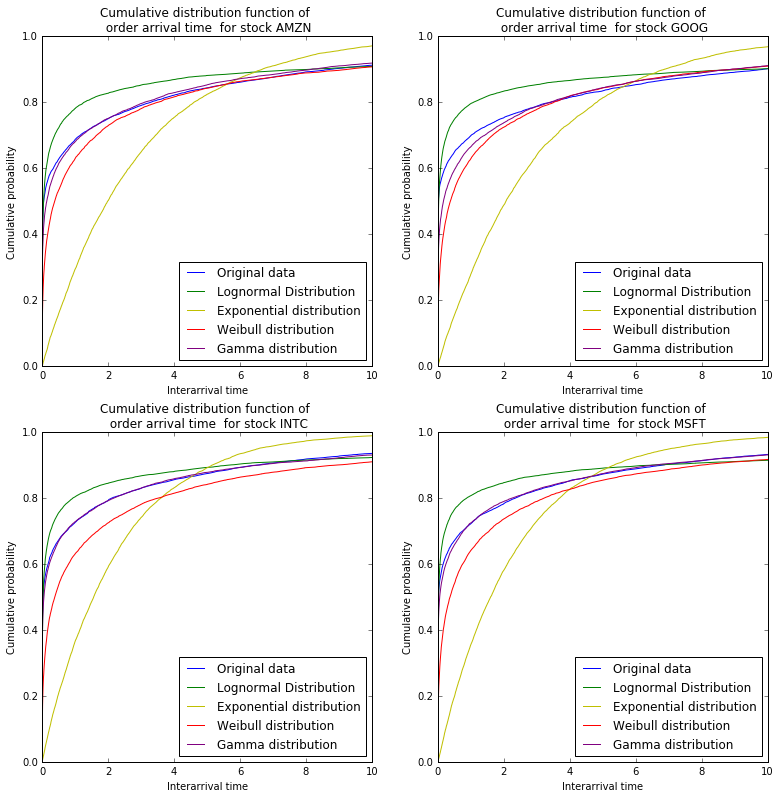
\includegraphics[width=6in,height=6in]{figures/arrival_time.png}
  \end{center}
\caption{Cumulative distribution of inter-arrival time for stock: AMZN,GOOG,INTC and MSFT. In each panel,four distribution, Lognormal, Exponential Weibull and Gamma, are compared with the original dataset. x axis represents the inter-arrival time of market orders and y axis shows the cumulative probability } \label{fig:arrival}
\end{figure}


\subsection{Volume of orders}

 
